\documentclass[report.tex]{subfiles}
\begin{document}

\chapter{Excercise 1B:4th order system}
In this assignment a controller will be designed such that the first mass $m_1$ will respond to the input within reasonable bandwidth.\\

The differential equations for this system are given in \ref{eq:1b_dv_x1} and \ref{eq:1b_dv_x2}.

\begin{equation}
m_1\ddot{x} = \sum\nolimits{F_1} = F + d(x_2-x_1) + k(x_2-x_1)
\label{eq:1b_dv_x1}
\end{equation}
\begin{equation}
m_2\ddot{x} = \sum\nolimits{F_2} = d(x_1-x_2)+ k(x_1-x_2)
\label{eq:1b_dv_x2}
\end{equation}

\section{Laplace transformation}
Using Laplace and that $m=m_1=m_2$ this results in \ref{eq:1b_laplace_x1} \ref{eq:1b_laplace_x2}
\begin{equation}
H_1(s) = \frac{X_1(s)}{F(s)}  = \frac{1}{s^2}\frac{ms^2+ds+k}{m^2s^2+2mds+2mk}
\label{eq:1b_laplace_x1}	
\end{equation}
\begin{equation}
H_2(s) = \frac{X_2(s)}{F(s)} = \frac{1}{s^2}\frac{ds+k}{m^2s^2+2mds+2mk}
\label{eq:1b_laplace_x2}
\end{equation}

\section{Controller Design}
For this exercise a controller should be designed that can control the behavior of $x_1$. There fore only equation \ref{eq:1b_laplace_x1} will be used from now. The bode plot of the system is shown in figure \ref{fig:1B3_bode}

\begin{figure}[H] 
	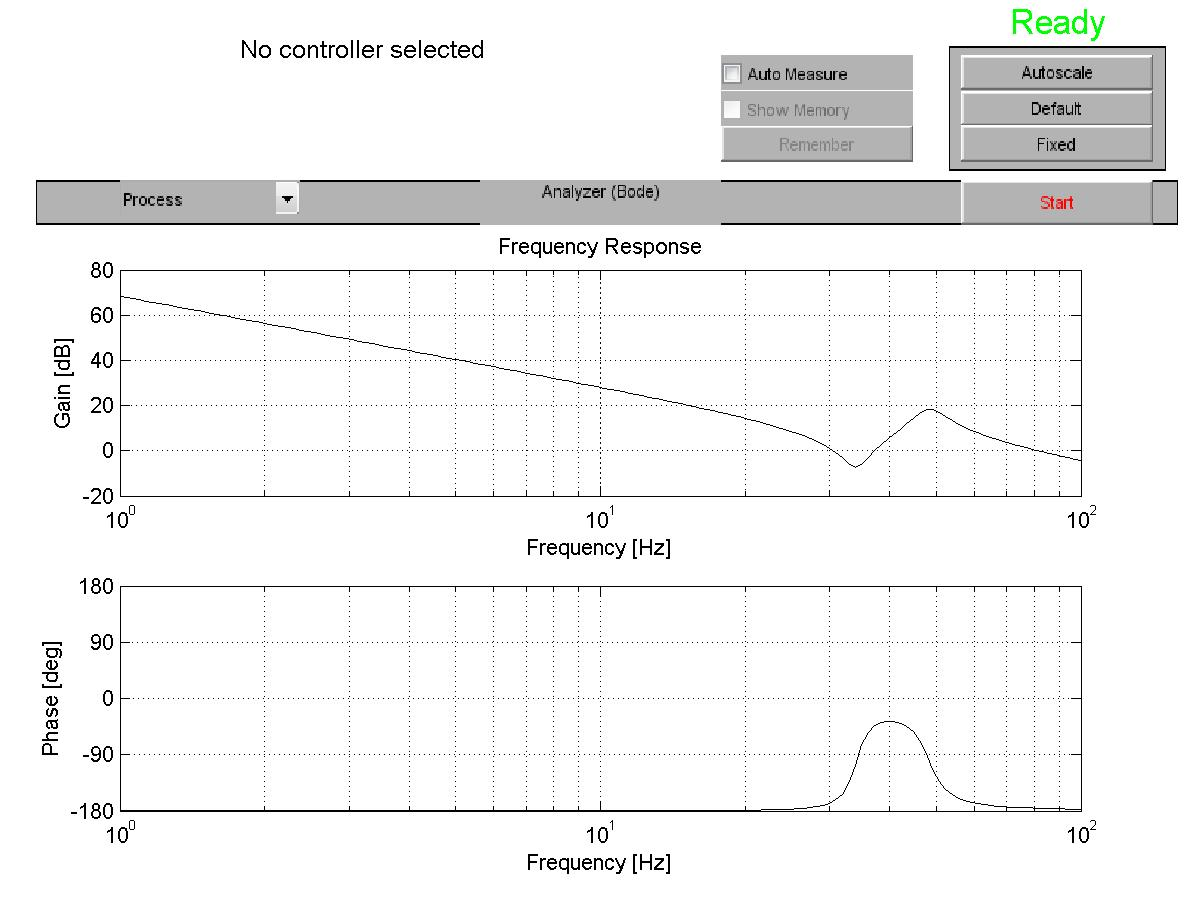
\includegraphics[width=0.8\textwidth]{1B3_bode}
	\centering
	\caption{Bode plot of $H_1(s)$}
	\label{fig:1B3_bode}
\end{figure}

For tuning the controller a certain bandwidth and phase margin must be chosen. 
Because there is no direct known application for the system a bandwidth of $30 Hz$ will be used as a rough estimate. This will filter any high frequency disturbances. A phase margin of $ 45\deg $ will be used, as it provides enough margin to the unstable region. 

If a controller of the form $C(s)=k_p+k_vs$ is chosen, the resulting transfer function $C(s)G(s)$ with $G(s)=H_1(s)$ will be equation \ref{eq:1b_openloop_x1}
\begin{equation}
C(s)G(s) = \frac{1}{s^2}\frac{(k_p+k_vs)(ms^2+ds+k)}{m^2s^2+2mds+2mk}
\label{eq:1b_openloop_x1}
\end{equation}

If one solves the equations \ref{eq:1b_openloop_x1_abs} and \ref{eq:1b_openloop_x1_arg} for $\omega = 2\pi f = 2\pi30 = 188.5 rad/s$, this results in valid values for $k_v$ and $k_p$. 

\begin{equation}
|C(j\omega)G(j\omega)| = |-\frac{1}{\omega^2}\frac{(k_p+k_vj\omega)(-m\omega^2+djw+k)}{-m^2\omega^2+2mdj\omega+2mk}| = 1
\label{eq:1b_openloop_x1_abs}
\end{equation}

\begin{equation}
arg(C(j\omega)G(j\omega)) = arg(-\frac{1}{\omega^2}\frac{(k_p+k_vj\omega)(-m\omega^2+djw+k)}{-m^2\omega^2+2mdj\omega+2mk}) = -135\deg
\label{eq:1b_openloop_x1_arg}
\end{equation}

As a result we get the following values. This results are checked with the Matlab diet toolbox and Matlab PID Design Tool:

\begin{equation}
	K_p=0.5968
\end{equation}
\begin{equation}
	K_d=.003407
\end{equation}

The bode plot for the open loop response $C(s)G(s)$ is shown in figure \ref{fig:1B3_bode_controller}

\begin{figure}[H] 
	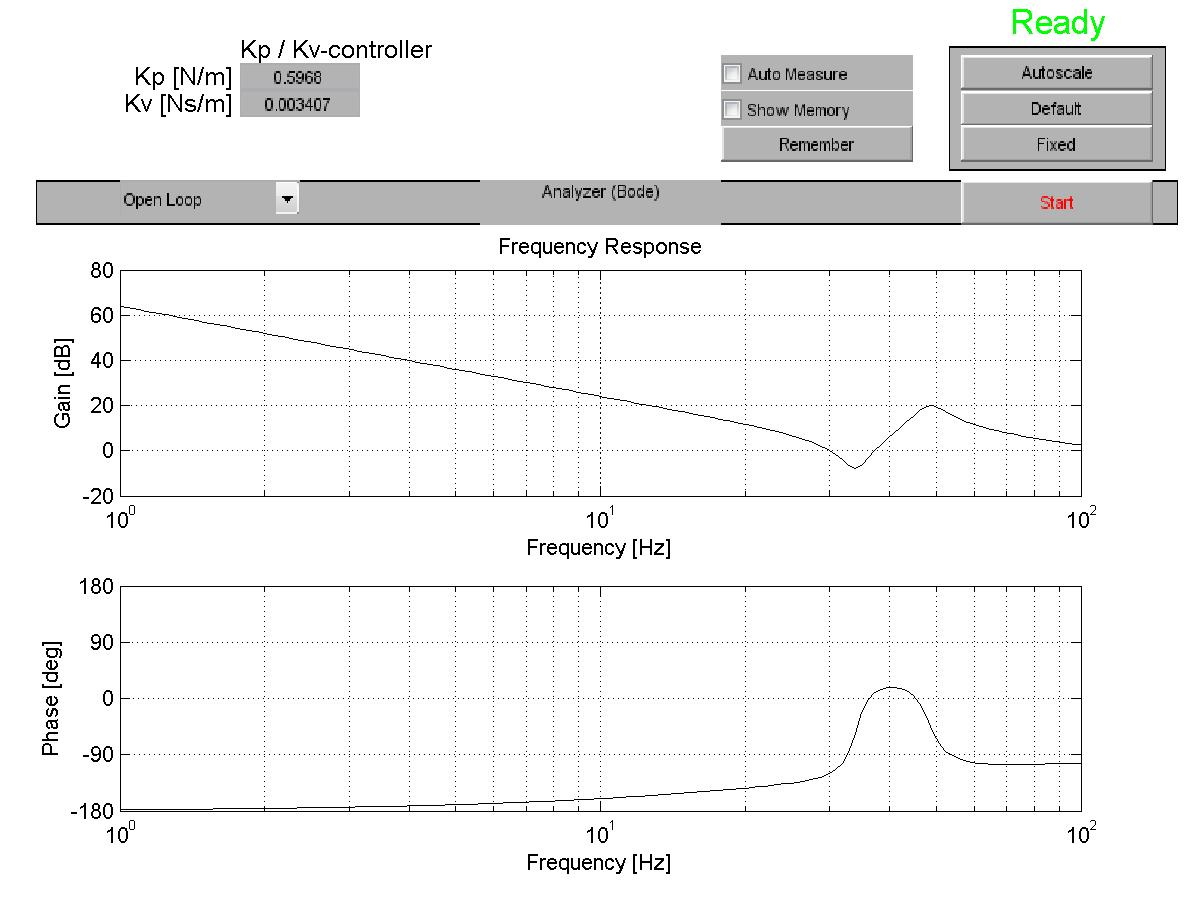
\includegraphics[width=0.8\textwidth]{1B3_bode_controller}
	\centering
	\caption{Bode plot of $C(s)G(s)$}
	\label{fig:1B3_bode_controller}
\end{figure}

\section{Evaluating Controller Performance}
If a closer look is taken at the Nyquist plot in figure \ref{fig:1B3_nyquist}, one can conclude that the system is stable. This results in the fact that there are 0 clockwise encirclements, and no poles or zeros within the contour of the plot. This means there are no right half plane poles and therefore the system is stable. 

\begin{figure}[H] 
	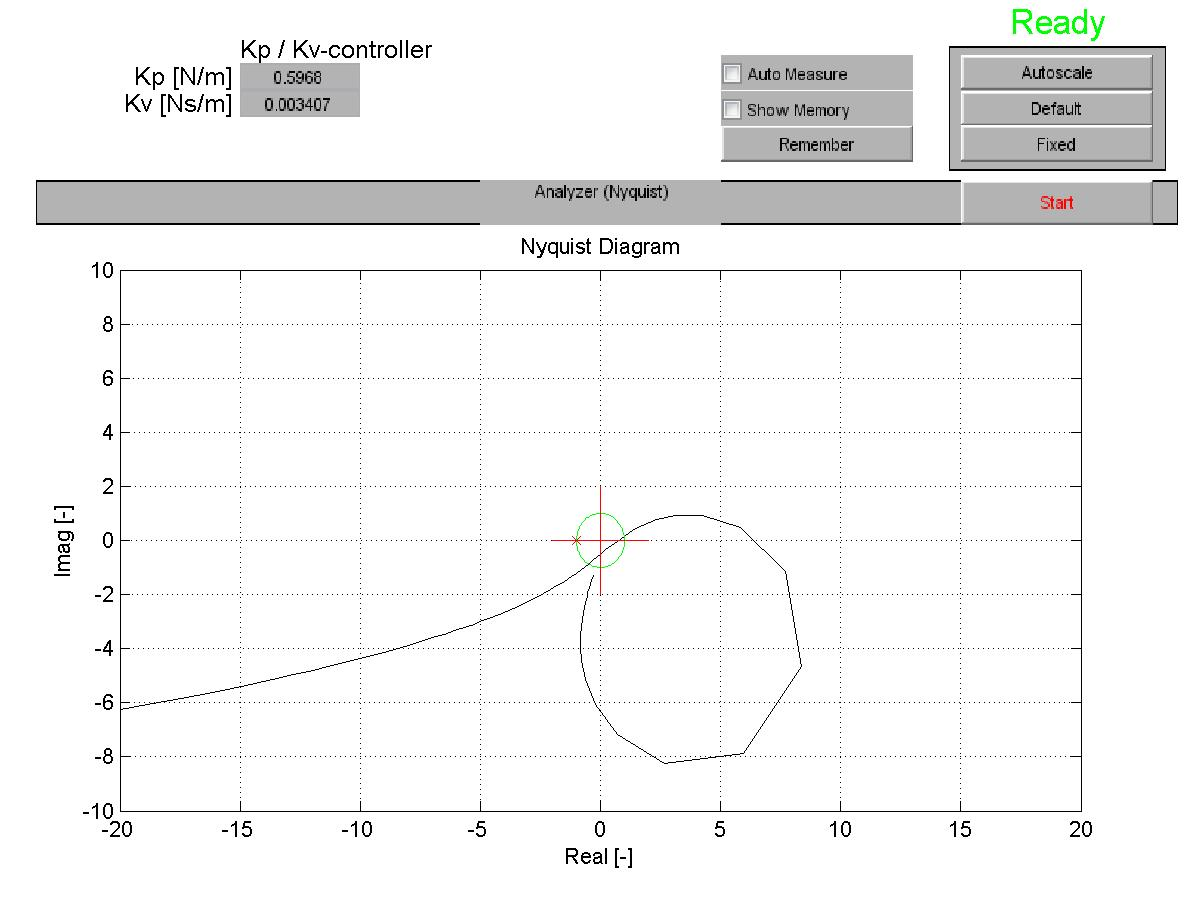
\includegraphics[width=0.8\textwidth]{1B3_nyquist}
	\centering
	\caption{Nyquist plot of $C(s)G(s)$}
	\label{fig:1B3_nyquist}
\end{figure}

However if a closer look is taken at the step response in figure \ref{fig:step30hz}, an overshoot and oscillation can be observed. These are both undesirable effects of choice of bandwidth. After some experimentation we have also seen cases without overshoot and oscillation. Noteworthy about this that it were cases with a value of 0 for $k_v$. This resulted in a bandwidth that was much higher and a response that was much faster. This faster response means lower rise and settling times. However, without an additional zero in the controller there will be an steady state error present. At the same time with larger bandwidths, one can ask question about properties as filtering and disturbance rejection. Therefore this gives a choice between fast response without overshoot and filtered system without steady state error. 

\begin{figure}[H] 
	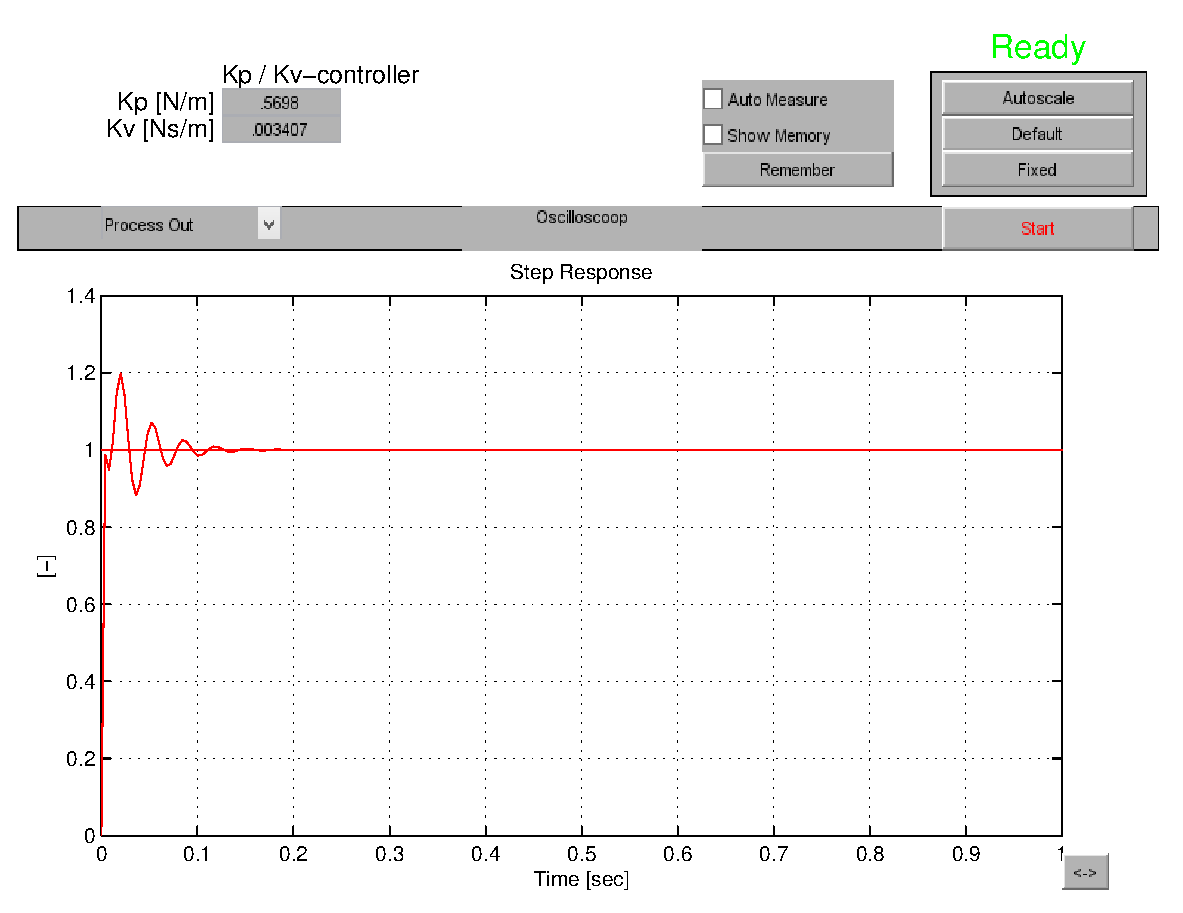
\includegraphics[width=0.8\textwidth]{step30hz.eps}
	\centering
	\caption{step response of the 30hz bandwitdth controller}
	\label{fig:step30hz}
\end{figure}

\end{document}
